\chapter{Arhitektura i dizajn sustava}
		
Naš sustav se može podijeliti na pet glavnih podsustava koji međusobno komuniciraju:
\begin{description}
	\item[Web preglednik:] Lokalno instalirani program koji omogućuje prikaz sadržaja sa interneta. 
	Pomoću tog programa korisnik može poslati zahtjeve za 
	resursima ili poslati neke podatke web poslužitelju. Web preglednik, 
	nakon što dobije zatražene informacije od web poslužitelja, korisniku prikazuje ssadržaj.

	\item[Web poslužitelj:] Centralni podsustav aplikacije koji obrađuje višestruke zahtjeve korisnika. To 
	može biti zasebno računalo ili samo softver. Komunikaciju s klijentima ostvaruje preko
	HTTP protokola. Web poslužitelj može, na korisnički zahtjev, poslati datoteke ili primiti
	neke podatke koje može spremiti u bazu podataka.

	\item[Baza podataka:] Koristi se za pohranjivanje podataka web apliakcije. Sastavljena je od tablica koje
	predstavljaju entitete s određenim atributima koji su međusobno povezani definiranim
	odnosima. Web aplikacija često komunicira s bazom, povlačeći i davajući podatke bazi.

	\item[Servis za obradu izgovora:] Vanjski servis pomoću kojeg ocjenjujemo izgovor stranih riječi korisnika. Web
	aplikacija komunicira sa servisom preko aplikacijskog sučelja (API).

	\item[Servis za riječi:] Vanjski servis pomoću kojeg administratori lakše stvaraju rječi i, samim time,
	rječnike. Servispreko aplikacijskog sučelja (API) pruža značenja riječi i 
	popratne pomoćne fraze koje olakšavaju proces učenja.
\end{description}

	
		

		

				
		\section{Baza podataka}
			
			\textbf{\textit{dio 1. revizije}}\\
			
		\textit{Potrebno je opisati koju vrstu i implementaciju baze podataka ste odabrali, glavne komponente od kojih se sastoji i slično.}
		
			\subsection{Opis tablica}
			

				\textit{Svaku tablicu je potrebno opisati po zadanom predlošku. Lijevo se nalazi točno ime varijable u bazi podataka, u sredini se nalazi tip podataka, a desno se nalazi opis varijable. Svjetlozelenom bojom označite primarni ključ. Svjetlo plavom označite strani ključ}
				
				
				\begin{longtblr}[
					label=none,
					entry=none
					]{
						width = \textwidth,
						colspec={|X[6,l]|X[6, l]|X[20, l]|}, 
						rowhead = 1,
					} %definicija širine tablice, širine stupaca, poravnanje i broja redaka naslova tablice
					\hline \SetCell[c=3]{c}{\textbf{korisnik - ime tablice}}	 \\ \hline[3pt]
					\SetCell{LightGreen}IDKorisnik & INT	&  	Lorem ipsum dolor sit amet, consectetur adipiscing elit, sed do eiusmod  	\\ \hline
					korisnickoIme	& VARCHAR &   	\\ \hline 
					email & VARCHAR &   \\ \hline 
					ime & VARCHAR	&  		\\ \hline 
					\SetCell{LightBlue} primjer	& VARCHAR &   	\\ \hline 
				\end{longtblr}
				
				
			
			\subsection{Dijagram baze podataka}
				\textit{ U ovom potpoglavlju potrebno je umetnuti dijagram baze podataka. Primarni i strani ključevi moraju biti označeni, a tablice povezane. Bazu podataka je potrebno normalizirati. Podsjetite se kolegija "Baze podataka".}

				\begin{figure}[H]
					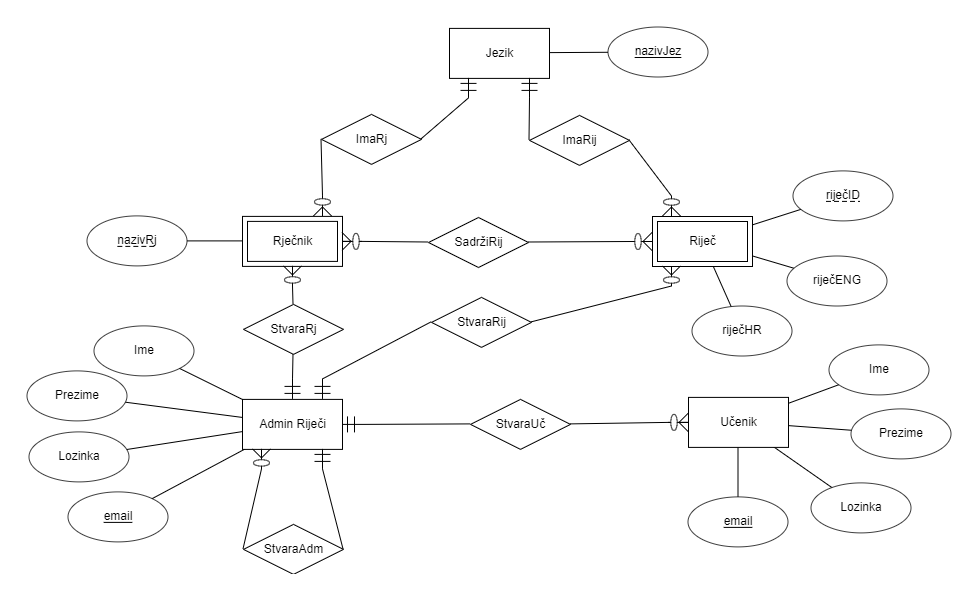
\includegraphics[scale=0.45]{dijagrami/ER_model_BP.png} 
					\centering
					\caption{ER model baze podataka}
					\label{fig:dijagram_ER-BP}
				\end{figure}
			
			\eject
			
			
		\section{Dijagram razreda}
		
			\textit{Potrebno je priložiti dijagram razreda s pripadajućim opisom. Zbog preglednosti je moguće dijagram razlomiti na više njih, ali moraju biti grupirani prema sličnim razinama apstrakcije i srodnim funkcionalnostima.}\\
			
			\textbf{\textit{dio 1. revizije}}\\
			
			\textit{Prilikom prve predaje projekta, potrebno je priložiti potpuno razrađen dijagram razreda vezan uz \textbf{generičku funkcionalnost} sustava. Ostale funkcionalnosti trebaju biti idejno razrađene u dijagramu sa sljedećim komponentama: nazivi razreda, nazivi metoda i vrste pristupa metodama (npr. javni, zaštićeni), nazivi atributa razreda, veze i odnosi između razreda.}\\
			
			\textbf{\textit{dio 2. revizije}}\\			
			
			\textit{Prilikom druge predaje projekta dijagram razreda i opisi moraju odgovarati stvarnom stanju implementacije}
			
			
			
			\eject
		
		\section{Dijagram stanja}
			
			
			\textbf{\textit{dio 2. revizije}}\\
			
			\textit{Potrebno je priložiti dijagram stanja i opisati ga. Dovoljan je jedan dijagram stanja koji prikazuje \textbf{značajan dio funkcionalnosti} sustava. Na primjer, stanja korisničkog sučelja i tijek korištenja neke ključne funkcionalnosti jesu značajan dio sustava, a registracija i prijava nisu. }
			
			
			\eject 
		
		\section{Dijagram aktivnosti}
			
			\textbf{\textit{dio 2. revizije}}\\
			
			 \textit{Potrebno je priložiti dijagram aktivnosti s pripadajućim opisom. Dijagram aktivnosti treba prikazivati značajan dio sustava.}
			
			\eject
		\section{Dijagram komponenti}
		
			\textbf{\textit{dio 2. revizije}}\\
		
			 \textit{Potrebno je priložiti dijagram komponenti s pripadajućim opisom. Dijagram komponenti treba prikazivati strukturu cijele aplikacije.}